\subsection{Động lực của bài toán}
Bộ não tự nhiên của con người được xem như là một cấu trúc mô-đun phức tạp với khả năng xử lý thông tin thông qua bộ phận ghi nhớ, kết hợp tri thức. Tính chất mô-đun đảm bảo rằng các tri thức được lưu trữ theo cách mà một mô-đun cụ thể sẽ không gây ảnh hưởng cho các mô-đun, chức năng khác của bộ não. Cấu trúc này của bộ não là một đặc tính quan trọng trong hệ thống sinh học tự nhiên và là động lực lớn trong việc phát triển các hệ thống trí tuế nhân tạo mô phỏng cấu trúc tương tự.

Mô hình mạng neural nhân tạo (thuật ngữ gốc: \emph{Artificial Neural Networks - ANN}) cũng được lấy cảm hứng từ ý tưởng về những cấu trúc lặp lại trong bộ não như vậy. Trong đó mạng với cấu trúc nhỏ hơn sẽ được sử dụng như là một phần của mạng có cấu trúc lớn hơn. Điều này thúc đấy một suy nghĩ rằng việc huấn luyện một mạng có cấu trúc nhỏ hơn sẽ có thể thúc đẩy độ hiệu quả khi huấn luyện những mạng có cấu trúc lớn hơn và ngược lại.
\begin{figure}[ht]
    \centering
    \fbox{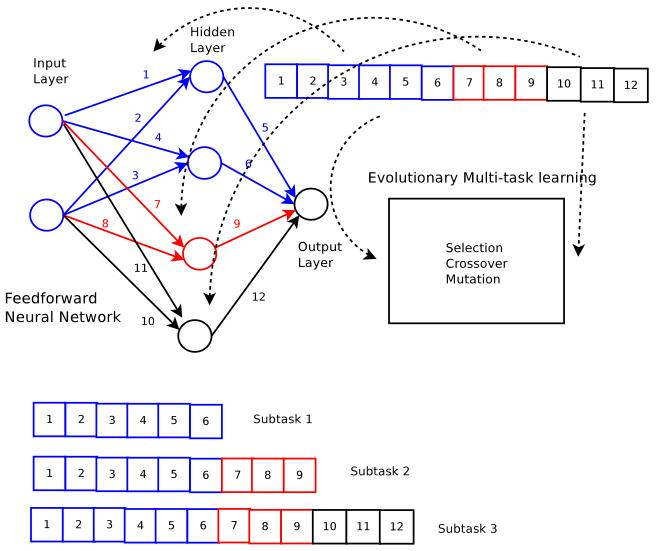
\includegraphics[width=0.75\linewidth]{modular-neural.jpg}}
    \caption{Mô hình biểu diễn mạng neural theo cấu trúc mô-đun hóa}
    \label{fig:problem:modular}
\end{figure}

Gần đây, nhóm nghiên cứu Gupta, Ong, and Feng tiếp tục phát triển mô hình MFO kết hợp với ý
tưởng của học có truyền đạt (thuật ngữ gốc: \emph{transfer learning}) \cite{pan2009survey} trở thành tối ưu hóa có truyền đạt (thuật ngữ gốc: \emph{transfer optimization}) \cite{gupta2017insights}. Mô hình tối ưu hóa có truyền đạt cho rằng ta có thể giải quyết 1 bài toán tối ưu hóa mới thông qua chính những tri thức từ những bài toán tối ưu hóa cũ. Họ sẽ duy trì một tập quần thể các cá thể tốt của những bài toán đã giải, đến khi gặp một bài toán mới, ta chỉ cần điều chỉnh lại các cá thể sẵn có thay vì phải giải lại bài toán đó từ đầu. Ý tưởng này có vẻ rất tự nhiên và hợp lý khi ngày nay chúng ta phải đối mặt với hàng núi dữ liệu học được cập nhật mỗi ngày. Việc huấn luyện lại từ đầu một mô hình cho tập dữ liệu mới đòi hỏi rất nhiều chi phí và công sức của các chuyên gia.

Giả sử trong bài toán nhận diện khuôn mặt với bộ dữ liệu đã được phân tích với các đặc tính (thuật ngữ gốc: \emph{features}). Một ANN đã được huấn luyện cho kết quả tối ưu có số lớp ẩn là $h$. Trong tương lai nếu có thêm nhiều điểm dữ liệu được thêm vào hoặc ta mở rộng phân tích thêm các đặc tính khác của dữ liệu thì có thể việc thay đổi cấu trúc mạng là cần thiết. Bởi vậy ta muốn thêm một số nút vào lớp ẩn để học mô hình ANN mới tương ứng với tập dữ liệu mới (lớn hơn tập dữ liệu cũ) mà vẫn sử dụng được những tri thức đã học từ mô hình trước đó. Có nghĩa là bộ tham số $(weight, bias)$ của mô hình trước vẫn được tái sử dụng theo một cách nào đó trong khi số lượng nút ở lớp ẩn tăng lên thành $h + n$. Với các phương pháp học mạng neural cơ bản thì nguy cơ cao rằng các tri thức đã học trước đó sẽ không được tận dụng khi cấu trúc mạng thay đổi. Bởi vậy ý tưởng mô-đun hóa mô hình mạng để đảm rằng tri thức được tái sử dụng hoặc chia sẻ tri thức cho những bài toán tương đương. 

\subsection{Phát biểu bài toán}
\subsubsection{Định nghĩa}
Trước khi đi vào bài toán, đồ án xin thống nhất ý nghĩa của một số ký hiệu sau:
\begin{itemize}
    \item $L$ là số lớp của ANN, các lớp được tính từ lớp ẩn đầu tiên (lớp đầu vào có thể được coi là lớp thứ 0). Nhận xét: ANN có $L$ lớp thì có $L-1$ lớp ẩn.
    \item Tham số lớp thứ $l \in {1,2,...L}$ gồm mà trận trọng số $W^{(l)}$,$l\in{1,2,...L}$ và véc-tơ độ lệch $b^{(l)}$.
    \item Số đơn vị xử lý của 1 lớp thứ $l$ được ký hiệu là $h_l$.
    \item Cấu hình lớp của ANN được ký hiệu theo bộ số thể hiện số đơn vị xử lý trên mỗi lớp kể từ lớp đầu vào (lớp 0). Ví dụ với \ref{fig:ann} là $H=(3,4,4,1)$. Ở dạng cấu hình ngắn gọn, ta có thể bỏ qua lớp đầu ra, chỉ quan tâm đến lớp ẩn và việt gọn thành $H=(4,4)$.
    \begin{figure}[h!] 
        \centering
        \fbox{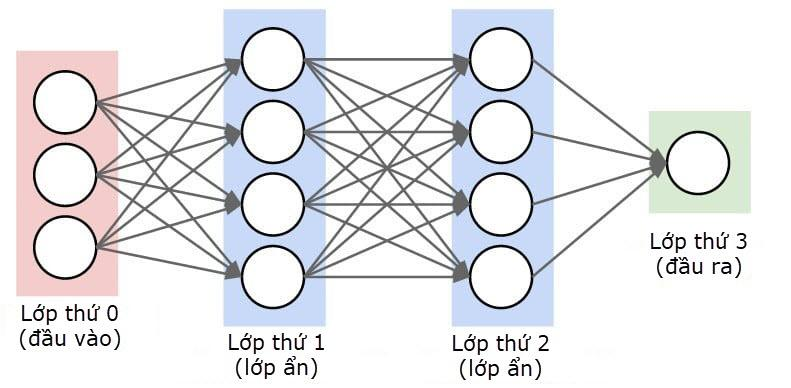
\includegraphics[width=0.7\linewidth]{thesis/images/ann.jpg}}
        \caption{Mạng neural 3 lớp gồm 2 lớp ẩn}
        \label{fig:ann}
    \end{figure}
    \item Kiểu gen của ANN được ký hiệu bằng véc-tơ D chiều $x$, $x[i], i\in {1,...,D}$ thể hiện biến thứ $i$ trong gen $x$, $x^{(p)}$ thể hiện cá thể thứ $p$ trong quần thể. Chỉ số dưới $x_i, x_j$ dùng để phân biệt 2 cá thể.
    \item $l,h \in \mathbb{R}$ tương ứng là cận dưới và cận trên cho mỗi biến trong kiểu gen $x$.
    \item $\mathcal{X}$ là kiểu hình của gen $x$. Trongnj số $W$ và độ lệch $b$ được phân tách ra từ kiểu hình $\mathcal{X}$. 
\end{itemize}
\subsubsection{Bài toán}
Bài toán có thể được phát biểu như sau:
\begin{itemize}
    \item \textbf{Đầu vào}: 
    \begin{itemize}
        \item $K$ tác vụ $T_1, T_2, ... ,T_k$ với $j \in [1,K]$. Mỗi tác vụ tương đương với một mô hình mạng neural có số lượng lớp ẩn và số lượng nút tại lớp ẩn khác.
        \item Mỗi tác vụ tương đương với một bài toán tối ưu hóa 1 cấu trúc mạng nơ-ron lần lượt là $h_1, h_2, ... , h_K$.
    \end{itemize}
    \item \textbf{Đầu ra}: $K$ tác vụ đã được tối ưu.
    \item \textbf{Mục tiêu}: Tìm ra bộ tham số tối ưu của mỗi cấu trúc mạng để tối thiểu hóa hàm lỗi trên mỗi tác vụ $T_j, j \in [1,K]$. 
\end{itemize}

\textit{Vậy làm thế nào để huấn luyện đồng thời nhiều ANN khác cấu trúc mà tận dụng được tri thức giữa các tác vụ?}
 
Như đã tôi trình bày trong chương \ref{mfea2}, thuật toán tiến hóa đa nhiệm có thể khai thác được mối quan hệ giữa các tác vụ có mối liên hệ với nhau bằng cách sử dụng một không gian biểu diễn chung. Với bài toán này mỗi một cấu trúc ANN sẽ được coi như là một tác vụ, các tác vụ có trúc nhỏ hơn sẽ trao đổi tri thức với tác vụ có cấu trúc lớn hơn thông qua mô hình của thuật toán tiến hóa đa nhiệm. 

Trong phạm vi chương này tôi sẽ trình bày ý tưởng đề xuất áp dụng tiến hóa đa nhiệm để giải mô hình các ANN khác cấu trúc, bên cạnh đó là một số nghiên cứu liên quan đến ý tưởng này.

